\section{oosalizer/graphs.c-Dateireferenz}
\label{graphs_8c}\index{oosalizer/graphs.c@{oosalizer/graphs.c}}
{\tt \#include $<$math.h$>$}\par
{\tt \#include $<$stdio.h$>$}\par
{\tt \#include $<$string.h$>$}\par
{\tt \#include $<$sys/types.h$>$}\par
{\tt \#include $<$gd.h$>$}\par
{\tt \#include $<$gdfontt.h$>$}\par
{\tt \#include $<$gdfonts.h$>$}\par
{\tt \#include $<$gdfontmb.h$>$}\par
{\tt \#include \char`\"{}webalizer.h\char`\"{}}\par
{\tt \#include \char`\"{}lang.h\char`\"{}}\par
{\tt \#include \char`\"{}graphs.h\char`\"{}}\par


Include-Abh\"{a}ngigkeitsdiagramm f\"{u}r graphs.c:\begin{figure}[H]
\begin{center}
\leavevmode
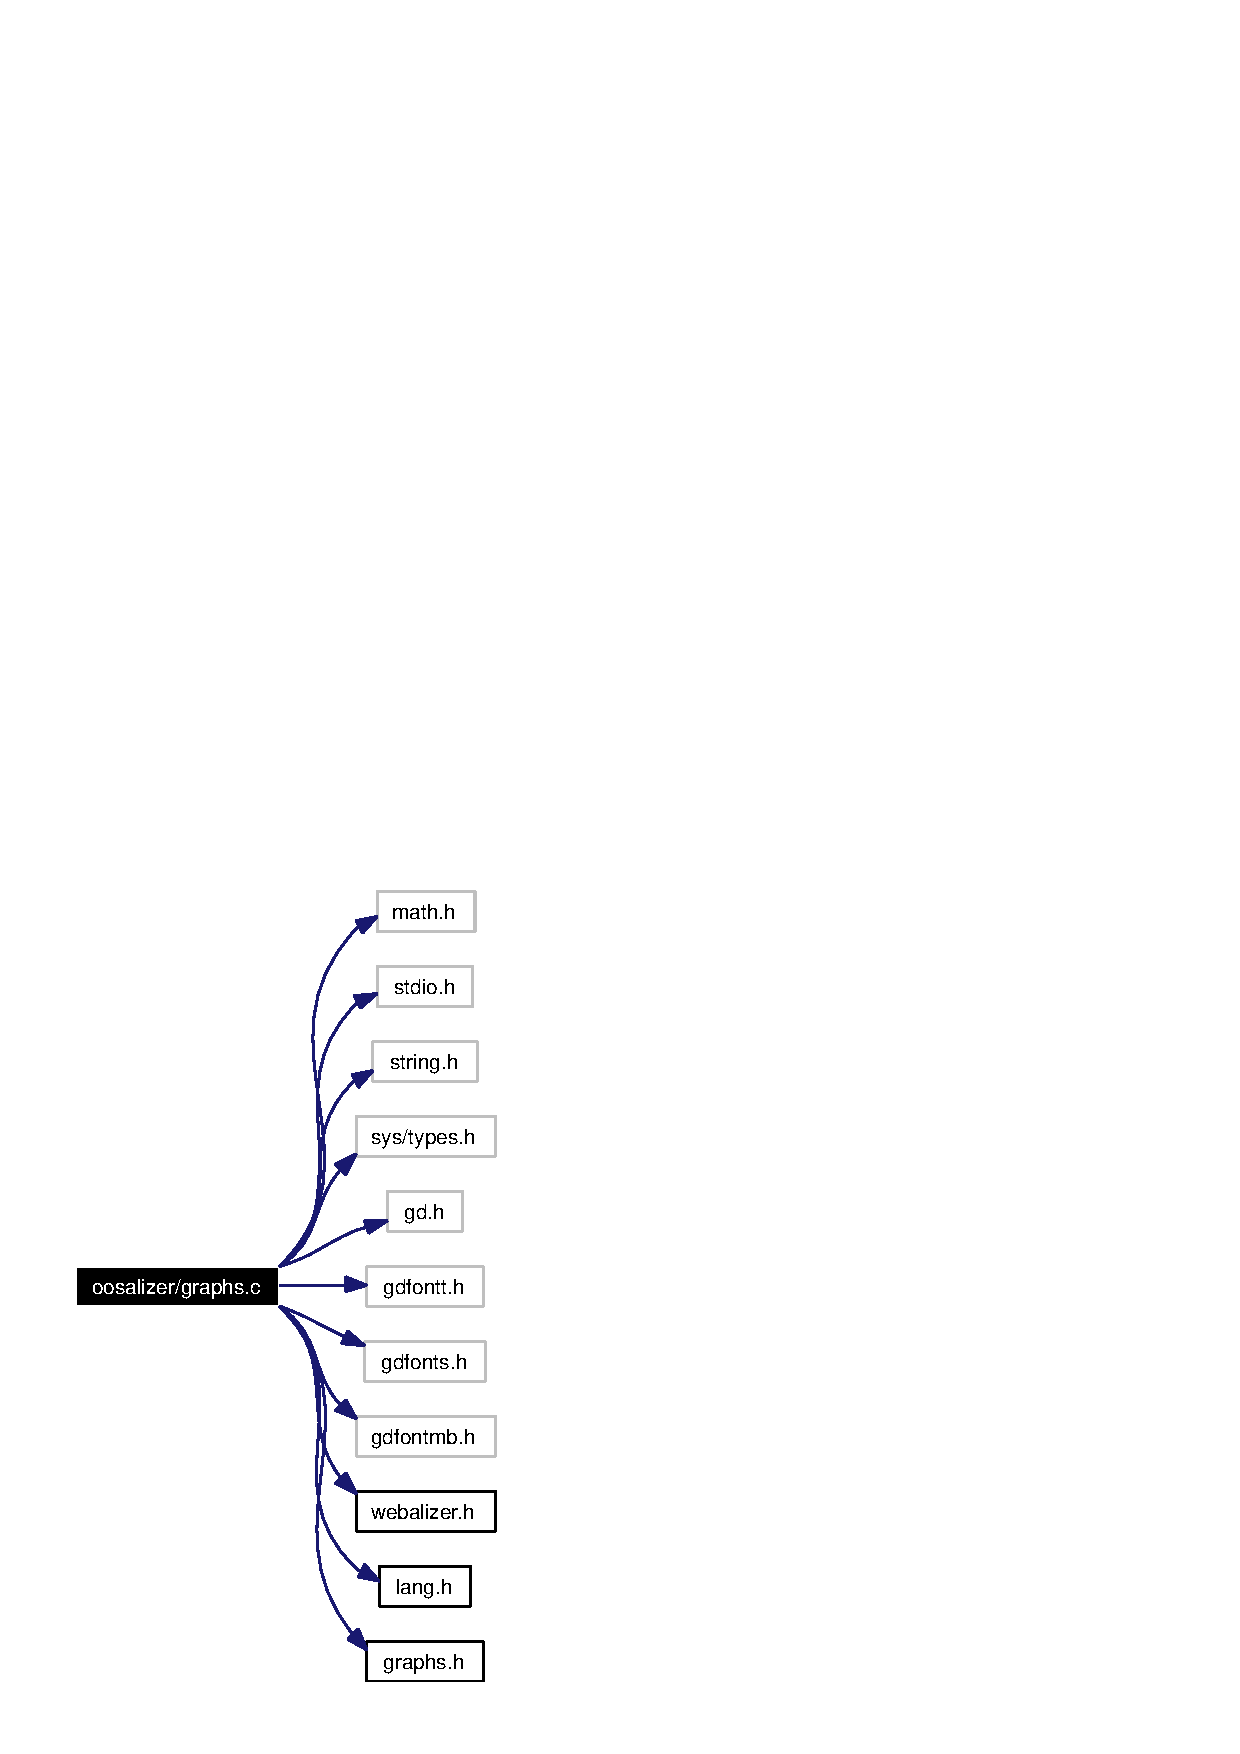
\includegraphics[width=119pt]{graphs_8c__incl}
\end{center}
\end{figure}
\subsection*{Datenstrukturen}
\begin{CompactItemize}
\item 
struct {\bf pie\_\-data}
\end{CompactItemize}
\subsection*{Makrodefinitionen}
\begin{CompactItemize}
\item 
\#define {\bf PI}~3.14159265358979323846
\item 
\#define {\bf COLOR1}~{\bf green}
\item 
\#define {\bf COLOR2}~{\bf blue}
\item 
\#define {\bf COLOR3}~{\bf orange}
\item 
\#define {\bf COLOR4}~{\bf red}
\item 
\#define {\bf COLOR5}~{\bf cyan}
\item 
\#define {\bf COLOR6}~{\bf yellow}
\item 
\#define {\bf CX}~156
\item 
\#define {\bf CY}~150
\item 
\#define {\bf XRAD}~240
\item 
\#define {\bf YRAD}~200
\item 
\#define {\bf YSIZE}~400
\end{CompactItemize}
\subsection*{Funktionen}
\begin{CompactItemize}
\item 
void {\bf init\_\-graph} (char $\ast$, int, int)
\item 
{\bf pie\_\-data} $\ast$ {\bf calc\_\-arc} (float, float)
\item 
int {\bf year\_\-graph6x} (char $\ast$fname, char $\ast$title, int fmonth, u\_\-long data1[12], u\_\-long data2[12], u\_\-long data3[12], double data4[12], u\_\-long data5[12], u\_\-long data6[12])
\item 
int {\bf month\_\-graph6} (char $\ast$fname, char $\ast$title, int month, int year, u\_\-long data1[31], u\_\-long data2[31], u\_\-long data3[31], double data4[31], u\_\-long data5[31], u\_\-long data6[31])
\item 
int {\bf day\_\-graph3} (char $\ast$fname, char $\ast$title, u\_\-long data1[24], u\_\-long data2[24], u\_\-long data3[24])
\item 
int {\bf pie\_\-chart} (char $\ast$fname, char $\ast$title, u\_\-long t\_\-val, u\_\-long data1[$\,$], char $\ast$legend[$\,$])
\end{CompactItemize}
\subsection*{Variablen}
\begin{CompactItemize}
\item 
char $\ast$ {\bf numchar} [$\,$]
\item 
gd\-Image\-Ptr {\bf im}
\item 
FILE $\ast$ {\bf out}
\item 
char {\bf maxvaltxt} [32]
\item 
float {\bf percent}
\item 
u\_\-long {\bf julday}
\item 
int {\bf black}
\item 
int {\bf white}
\item 
int {\bf grey}
\item 
int {\bf dkgrey}
\item 
int {\bf red}
\item 
int {\bf blue}
\item 
int {\bf orange}
\item 
int {\bf green}
\item 
int {\bf cyan}
\item 
int {\bf yellow}
\end{CompactItemize}


\subsection{Makro-Dokumentation}
\index{graphs.c@{graphs.c}!COLOR1@{COLOR1}}
\index{COLOR1@{COLOR1}!graphs.c@{graphs.c}}
\subsubsection{\setlength{\rightskip}{0pt plus 5cm}\#define COLOR1~{\bf green}}\label{graphs_8c_1169cd1b397420b29bd3b0153f047818}




Definiert in Zeile 47 der Datei graphs.c.

Wird benutzt von month\_\-graph6().\index{graphs.c@{graphs.c}!COLOR2@{COLOR2}}
\index{COLOR2@{COLOR2}!graphs.c@{graphs.c}}
\subsubsection{\setlength{\rightskip}{0pt plus 5cm}\#define COLOR2~{\bf blue}}\label{graphs_8c_609e0791889f4cde446ee0eb6efd369a}




Definiert in Zeile 48 der Datei graphs.c.\index{graphs.c@{graphs.c}!COLOR3@{COLOR3}}
\index{COLOR3@{COLOR3}!graphs.c@{graphs.c}}
\subsubsection{\setlength{\rightskip}{0pt plus 5cm}\#define COLOR3~{\bf orange}}\label{graphs_8c_299edc84540341c664cd7a183e8fc9bd}




Definiert in Zeile 49 der Datei graphs.c.\index{graphs.c@{graphs.c}!COLOR4@{COLOR4}}
\index{COLOR4@{COLOR4}!graphs.c@{graphs.c}}
\subsubsection{\setlength{\rightskip}{0pt plus 5cm}\#define COLOR4~{\bf red}}\label{graphs_8c_5b1074ec004e850c360022e0d433e475}




Definiert in Zeile 50 der Datei graphs.c.\index{graphs.c@{graphs.c}!COLOR5@{COLOR5}}
\index{COLOR5@{COLOR5}!graphs.c@{graphs.c}}
\subsubsection{\setlength{\rightskip}{0pt plus 5cm}\#define COLOR5~{\bf cyan}}\label{graphs_8c_b1b154af4927f41dc0ac230992bf1a15}




Definiert in Zeile 51 der Datei graphs.c.\index{graphs.c@{graphs.c}!COLOR6@{COLOR6}}
\index{COLOR6@{COLOR6}!graphs.c@{graphs.c}}
\subsubsection{\setlength{\rightskip}{0pt plus 5cm}\#define COLOR6~{\bf yellow}}\label{graphs_8c_8fd4fb399b4659d7aed1fcb5cc182ebb}




Definiert in Zeile 52 der Datei graphs.c.\index{graphs.c@{graphs.c}!CX@{CX}}
\index{CX@{CX}!graphs.c@{graphs.c}}
\subsubsection{\setlength{\rightskip}{0pt plus 5cm}\#define CX~156}\label{graphs_8c_0b4c12a5dc8490a3cff8385334db2d13}




Definiert in Zeile 54 der Datei graphs.c.

Wird benutzt von calc\_\-arc() und pie\_\-chart().\index{graphs.c@{graphs.c}!CY@{CY}}
\index{CY@{CY}!graphs.c@{graphs.c}}
\subsubsection{\setlength{\rightskip}{0pt plus 5cm}\#define CY~150}\label{graphs_8c_c5bc792e372b15e7a1d3efe6daac9aec}




Definiert in Zeile 55 der Datei graphs.c.

Wird benutzt von calc\_\-arc() und pie\_\-chart().\index{graphs.c@{graphs.c}!PI@{PI}}
\index{PI@{PI}!graphs.c@{graphs.c}}
\subsubsection{\setlength{\rightskip}{0pt plus 5cm}\#define PI~3.14159265358979323846}\label{graphs_8c_598a3330b3c21701223ee0ca14316eca}




Definiert in Zeile 44 der Datei graphs.c.

Wird benutzt von calc\_\-arc().\index{graphs.c@{graphs.c}!XRAD@{XRAD}}
\index{XRAD@{XRAD}!graphs.c@{graphs.c}}
\subsubsection{\setlength{\rightskip}{0pt plus 5cm}\#define XRAD~240}\label{graphs_8c_e1eec295ea8cd8f04c1f24b59110fcae}




Definiert in Zeile 56 der Datei graphs.c.

Wird benutzt von calc\_\-arc() und pie\_\-chart().\index{graphs.c@{graphs.c}!YRAD@{YRAD}}
\index{YRAD@{YRAD}!graphs.c@{graphs.c}}
\subsubsection{\setlength{\rightskip}{0pt plus 5cm}\#define YRAD~200}\label{graphs_8c_3eeb4d5b339574d992e5ac5b2c5cd8ff}




Definiert in Zeile 57 der Datei graphs.c.

Wird benutzt von calc\_\-arc() und pie\_\-chart().\index{graphs.c@{graphs.c}!YSIZE@{YSIZE}}
\index{YSIZE@{YSIZE}!graphs.c@{graphs.c}}
\subsubsection{\setlength{\rightskip}{0pt plus 5cm}\#define YSIZE~400}\label{graphs_8c_faefa0d521156ca605f526c14d05e272}




Definiert in Zeile 296 der Datei graphs.c.

\subsection{Dokumentation der Funktionen}
\index{graphs.c@{graphs.c}!calc_arc@{calc\_\-arc}}
\index{calc_arc@{calc\_\-arc}!graphs.c@{graphs.c}}
\subsubsection{\setlength{\rightskip}{0pt plus 5cm}struct {\bf pie\_\-data} $\ast$ calc\_\-arc (float, float)}\label{graphs_8c_b831d5a0b0198ea523e0b116aaa20488}




Definiert in Zeile 694 der Datei graphs.c.

Benutzt CX, CY, pie\_\-data::mx, pie\_\-data::my, PI, pie\_\-data::x, XRAD, pie\_\-data::y und YRAD.

Wird benutzt von pie\_\-chart().\index{graphs.c@{graphs.c}!day_graph3@{day\_\-graph3}}
\index{day_graph3@{day\_\-graph3}!graphs.c@{graphs.c}}
\subsubsection{\setlength{\rightskip}{0pt plus 5cm}int day\_\-graph3 (char $\ast$ {\em fname}, char $\ast$ {\em title}, u\_\-long {\em data1}[24], u\_\-long {\em data2}[24], u\_\-long {\em data3}[24])}\label{graphs_8c_98296b41d7e2982e4b341e6ed18255ac}




Definiert in Zeile 503 der Datei graphs.c.

Benutzt black, dkgrey, graph\_\-lines, im, init\_\-graph() und numchar.

Wird benutzt von write\_\-month\_\-html().\index{graphs.c@{graphs.c}!init_graph@{init\_\-graph}}
\index{init_graph@{init\_\-graph}!graphs.c@{graphs.c}}
\subsubsection{\setlength{\rightskip}{0pt plus 5cm}void init\_\-graph (char $\ast$, int, int)}\label{graphs_8c_2040d817b934e470b4a2cdeb9811c097}




Definiert in Zeile 716 der Datei graphs.c.

Benutzt black, blue, cyan, dkgrey, green, grey, im, orange, red, white und yellow.

Wird benutzt von day\_\-graph3(), month\_\-graph6(), pie\_\-chart() und year\_\-graph6x().\index{graphs.c@{graphs.c}!month_graph6@{month\_\-graph6}}
\index{month_graph6@{month\_\-graph6}!graphs.c@{graphs.c}}
\subsubsection{\setlength{\rightskip}{0pt plus 5cm}int month\_\-graph6 (char $\ast$ {\em fname}, char $\ast$ {\em title}, int {\em month}, int {\em year}, u\_\-long {\em data1}[31], u\_\-long {\em data2}[31], u\_\-long {\em data3}[31], double {\em data4}[31], u\_\-long {\em data5}[31], u\_\-long {\em data6}[31])}\label{graphs_8c_7d33e4e14ae660bf05b5793f8e18d091}




Definiert in Zeile 298 der Datei graphs.c.

Benutzt black, COLOR1, dkgrey, graph\_\-lines, im, init\_\-graph(), jdate(), julday, numchar und white.

Wird benutzt von write\_\-month\_\-html().\index{graphs.c@{graphs.c}!pie_chart@{pie\_\-chart}}
\index{pie_chart@{pie\_\-chart}!graphs.c@{graphs.c}}
\subsubsection{\setlength{\rightskip}{0pt plus 5cm}int pie\_\-chart (char $\ast$ {\em fname}, char $\ast$ {\em title}, u\_\-long {\em t\_\-val}, u\_\-long {\em data1}[$\,$], char $\ast$ {\em legend}[$\,$])}\label{graphs_8c_49e615d9104950eeb7a886df4301f7da}




Definiert in Zeile 610 der Datei graphs.c.

Benutzt black, buffer, calc\_\-arc(), CX, CY, im, init\_\-graph(), percent, pie\_\-data::x, XRAD, pie\_\-data::y und YRAD.\index{graphs.c@{graphs.c}!year_graph6x@{year\_\-graph6x}}
\index{year_graph6x@{year\_\-graph6x}!graphs.c@{graphs.c}}
\subsubsection{\setlength{\rightskip}{0pt plus 5cm}int year\_\-graph6x (char $\ast$ {\em fname}, char $\ast$ {\em title}, int {\em fmonth}, u\_\-long {\em data1}[12], u\_\-long {\em data2}[12], u\_\-long {\em data3}[12], double {\em data4}[12], u\_\-long {\em data5}[12], u\_\-long {\em data6}[12])}\label{graphs_8c_58eec29feb4d1c90de8813c8c59d4fcd}




Definiert in Zeile 88 der Datei graphs.c.

Benutzt black, dkgrey, graph\_\-lines, im, init\_\-graph(), s\_\-month und white.

\subsection{Variablen-Dokumentation}
\index{graphs.c@{graphs.c}!black@{black}}
\index{black@{black}!graphs.c@{graphs.c}}
\subsubsection{\setlength{\rightskip}{0pt plus 5cm}int {\bf black}}\label{graphs_8c_8784d4f8ed73cff78355d2ed8e0c3a3b}




Definiert in Zeile 79 der Datei graphs.c.

Wird benutzt von day\_\-graph3(), init\_\-graph(), month\_\-graph6(), pie\_\-chart() und year\_\-graph6x().\index{graphs.c@{graphs.c}!blue@{blue}}
\index{blue@{blue}!graphs.c@{graphs.c}}
\subsubsection{\setlength{\rightskip}{0pt plus 5cm}int {\bf blue}}\label{graphs_8c_16043f28bf0a6b55db852853f0683fc2}




Definiert in Zeile 79 der Datei graphs.c.

Wird benutzt von init\_\-graph().\index{graphs.c@{graphs.c}!cyan@{cyan}}
\index{cyan@{cyan}!graphs.c@{graphs.c}}
\subsubsection{\setlength{\rightskip}{0pt plus 5cm}int {\bf cyan}}\label{graphs_8c_f6bc84de5c6f5361f222772133cf1ab8}




Definiert in Zeile 79 der Datei graphs.c.

Wird benutzt von init\_\-graph().\index{graphs.c@{graphs.c}!dkgrey@{dkgrey}}
\index{dkgrey@{dkgrey}!graphs.c@{graphs.c}}
\subsubsection{\setlength{\rightskip}{0pt plus 5cm}int {\bf dkgrey}}\label{graphs_8c_ee1005868568d9750214235693ba63e1}




Definiert in Zeile 79 der Datei graphs.c.

Wird benutzt von day\_\-graph3(), init\_\-graph(), month\_\-graph6() und year\_\-graph6x().\index{graphs.c@{graphs.c}!green@{green}}
\index{green@{green}!graphs.c@{graphs.c}}
\subsubsection{\setlength{\rightskip}{0pt plus 5cm}int {\bf green}}\label{graphs_8c_6e208843f894f38fa7644608917a2a41}




Definiert in Zeile 79 der Datei graphs.c.

Wird benutzt von init\_\-graph().\index{graphs.c@{graphs.c}!grey@{grey}}
\index{grey@{grey}!graphs.c@{graphs.c}}
\subsubsection{\setlength{\rightskip}{0pt plus 5cm}int {\bf grey}}\label{graphs_8c_852d2c8c77477e510b44d799fdaaf1f9}




Definiert in Zeile 79 der Datei graphs.c.

Wird benutzt von init\_\-graph().\index{graphs.c@{graphs.c}!im@{im}}
\index{im@{im}!graphs.c@{graphs.c}}
\subsubsection{\setlength{\rightskip}{0pt plus 5cm}gd\-Image\-Ptr {\bf im}}\label{graphs_8c_0e84b6d886b70b0cf21c56e5e26f0ed9}




Definiert in Zeile 70 der Datei graphs.c.

Wird benutzt von day\_\-graph3(), init\_\-graph(), month\_\-graph6(), pie\_\-chart() und year\_\-graph6x().\index{graphs.c@{graphs.c}!julday@{julday}}
\index{julday@{julday}!graphs.c@{graphs.c}}
\subsubsection{\setlength{\rightskip}{0pt plus 5cm}u\_\-long {\bf julday}}\label{graphs_8c_488cb40243821792a9a226ca1042b3e1}




Definiert in Zeile 74 der Datei graphs.c.

Wird benutzt von month\_\-graph6().\index{graphs.c@{graphs.c}!maxvaltxt@{maxvaltxt}}
\index{maxvaltxt@{maxvaltxt}!graphs.c@{graphs.c}}
\subsubsection{\setlength{\rightskip}{0pt plus 5cm}char {\bf maxvaltxt}[32]}\label{graphs_8c_3933b61d12d9878aa33d711259d94c5f}




Definiert in Zeile 72 der Datei graphs.c.\index{graphs.c@{graphs.c}!numchar@{numchar}}
\index{numchar@{numchar}!graphs.c@{graphs.c}}
\subsubsection{\setlength{\rightskip}{0pt plus 5cm}char$\ast$ {\bf numchar}[$\,$]}\label{graphs_8c_d8920ceda92347671d37ba01be631d65}


{\bf Initialisierung:}

\footnotesize\begin{verbatim} { " 0"," 1"," 2"," 3"," 4"," 5"," 6"," 7"," 8"," 9","10",
                    "11","12","13","14","15","16","17","18","19","20",
                    "21","22","23","24","25","26","27","28","29","30","31"}
\end{verbatim}\normalsize 


Definiert in Zeile 66 der Datei graphs.c.

Wird benutzt von day\_\-graph3() und month\_\-graph6().\index{graphs.c@{graphs.c}!orange@{orange}}
\index{orange@{orange}!graphs.c@{graphs.c}}
\subsubsection{\setlength{\rightskip}{0pt plus 5cm}int {\bf orange}}\label{graphs_8c_d316f80317cb97c5ada72ac0e05bbf92}




Definiert in Zeile 79 der Datei graphs.c.

Wird benutzt von init\_\-graph().\index{graphs.c@{graphs.c}!out@{out}}
\index{out@{out}!graphs.c@{graphs.c}}
\subsubsection{\setlength{\rightskip}{0pt plus 5cm}FILE$\ast$ {\bf out}}\label{graphs_8c_1277960b5f2b37137fe9b0b5a1ea0beb}




Definiert in Zeile 71 der Datei graphs.c.\index{graphs.c@{graphs.c}!percent@{percent}}
\index{percent@{percent}!graphs.c@{graphs.c}}
\subsubsection{\setlength{\rightskip}{0pt plus 5cm}float {\bf percent}}\label{graphs_8c_ac167f3972a2f244f4b32c8ee5b89364}




Definiert in Zeile 73 der Datei graphs.c.

Wird benutzt von pie\_\-chart().\index{graphs.c@{graphs.c}!red@{red}}
\index{red@{red}!graphs.c@{graphs.c}}
\subsubsection{\setlength{\rightskip}{0pt plus 5cm}int {\bf red}}\label{graphs_8c_6761340706096510fd89edca40a63b9b}




Definiert in Zeile 79 der Datei graphs.c.

Wird benutzt von init\_\-graph().\index{graphs.c@{graphs.c}!white@{white}}
\index{white@{white}!graphs.c@{graphs.c}}
\subsubsection{\setlength{\rightskip}{0pt plus 5cm}int {\bf white}}\label{graphs_8c_52b8a1dc217164197e6e5ba60ec911bf}




Definiert in Zeile 79 der Datei graphs.c.

Wird benutzt von init\_\-graph(), month\_\-graph6() und year\_\-graph6x().\index{graphs.c@{graphs.c}!yellow@{yellow}}
\index{yellow@{yellow}!graphs.c@{graphs.c}}
\subsubsection{\setlength{\rightskip}{0pt plus 5cm}int {\bf yellow}}\label{graphs_8c_34167711871149458e41ef5d3e3541fe}




Definiert in Zeile 79 der Datei graphs.c.

Wird benutzt von init\_\-graph().